\documentclass[conference]{IEEEtran}
\usepackage{amsmath,amssymb,amsthm}
\usepackage[T1]{fontenc}
\usepackage{booktabs}
\usepackage{graphicx}
\usepackage{algorithm}
\usepackage{algpseudocode}
\usepackage{hyperref}
\hypersetup{hidelinks}
\newtheorem{proposition}{Proposition}
\newtheorem{lemma}{Lemma}
\newcommand{\Oh}{\mathcal{O}}
\title{The Representation Technique Speeds Up\\
Subset Sum Only on Random Inputs}
\author{\IEEEauthorblockN{Le Duc Minh}
\IEEEauthorblockA{\href{mailto:minh.leduc.0210@gmail.com}{minh.leduc.0210@gmail.com}}}
\begin{document}
\maketitle
\begin{abstract}
Meet-in-the-middle solves subset sum in about $2^{n/2}$ steps on every input.
On random inputs, a family of methods called the \emph{representation
technique} does much better, about $2^{0.291n}$. This note explains the
technique to readers who know meet-in-the-middle, and asks why its speed has
not been carried over to every input. We work through a small example, derive
the basic cost formula, and recompute the published exponents of
Howgrave-Graham and Joux ($0.337$) and of Becker, Coron and Joux ($0.291$) from
their cost models. We then report two small experiments that rule out two
natural explanations for the gap between random and worst-case inputs.
Finally we prove that the three coefficient sets left open by the recent
worst-case work of Randolph and W\k{e}grzycki, namely $\{0,1\}$, $\{-1,1\}$ and
$\{-2,-1,1,2\}$, cannot be written as a sum of two sets in which some
coefficient appears twice, which is the property their method relies on. Plain
subset sum is the case $\{0,1\}$. We do not claim a faster worst-case
algorithm.
\end{abstract}
\begin{IEEEkeywords}
subset sum, knapsack, representation technique, meet-in-the-middle,
worst-case analysis
\end{IEEEkeywords}

\section{Introduction}
Given integers $a_1,\dots,a_n$ and a target $b$, subset sum asks whether some of
the $a_i$ add up to $b$. The standard fast method, meet-in-the-middle of
Horowitz and Sahni~\cite{hs}, splits the numbers into a left and a right half,
lists the $2^{n/2}$ subset sums of each half, and looks for one sum from each
side that together give $b$. It takes about $2^{n/2}$ steps on every input.
Schroeppel and Shamir~\cite{ss} reduced the memory to about $2^{n/4}$, and Chen,
Jin, Randolph and Servedio~\cite{chen} removed a polynomial factor from the
time, but no method is known that beats $2^{(1/2-\varepsilon)n}$ on every input.

In 2010 Howgrave-Graham and Joux~\cite{hgj} found a different way to cut the
search. Instead of fixing one split of the \emph{positions} into left and right,
they split the \emph{answer} into two smaller pieces, and use the fact that an
answer can be split in a huge number of ways. On random inputs whose numbers
have about $n$ bits each, their method runs in about $2^{0.337n}$ steps. Becker,
Coron and Joux~\cite{bcj} pushed this to about $2^{0.291n}$. Both analyses assume
that the input behaves like a random one. For a carefully chosen input this can
fail, so neither result gives a bound that holds for every input.

Randolph and W\k{e}grzycki~\cite{rw} recently made a version of the technique
work on every input for a large class of related problems. Three cases resisted,
and plain subset sum is one of them.

\subsection{What this note does}
\begin{itemize}
\item Section~\ref{sec:prelim} collects the notation and the few facts about
counting and modular arithmetic that the rest uses.
\item Section~\ref{sec:idea} explains the representation idea with a small
example and derives its basic cost.
\item Section~\ref{sec:published} recomputes the published exponents of
\cite{hgj} and \cite{bcj} from their cost models.
\item Section~\ref{sec:probes} explains why these results are average-case, and
reports two experiments that rule out two possible reasons for the gap.
\item Section~\ref{sec:frontier} explains the worst-case method of~\cite{rw}
and proves that it has nothing to work with on the three open cases.
\end{itemize}
Derivations and proofs are in the appendices.

\section{Preliminaries}\label{sec:prelim}

\subsection{Solutions as 0/1 vectors}
A choice of numbers is a vector $x\in\{0,1\}^n$, where $x_i=1$ means that $a_i$
is chosen. Its sum is $a\cdot x=\sum_i a_ix_i$, and its \emph{weight} $|x|$ is
the number of chosen items. We write $\ell$ for the weight of a solution and
$\lambda=\ell/n$ for its fraction of the items. On random hard inputs a solution
usually has $\lambda\approx1/2$.

\subsection{Counting with entropy}
The number of ways to choose $k$ items out of $n$ is $\binom{n}{k}$. For
$k=pn$ there is a convenient estimate:
\[
\binom{n}{pn}=2^{H(p)\,n}\ \text{up to a polynomial factor},
\]
where $H(p)=-p\log_2 p-(1-p)\log_2(1-p)$ is the binary entropy. For example
$H(1/2)=1$ and $H(1/4)\approx0.811$, so there are about $2^{0.811n}$ subsets with
$n/4$ items. We use $\Oh^*(\cdot)$ and ``about'' to mean ``up to polynomial
factors in $n$''.

\subsection{Residues and filters}
For a positive integer $M$, the \emph{residue} of an integer $s$ is
$s\bmod M\in\{0,\dots,M-1\}$. A \emph{filter} keeps only the vectors whose sum has
one chosen residue $R$. If the sums are spread evenly over the $M$ residues, a
filter keeps about a $1/M$ fraction of them. Residues add: if
$a\cdot y\equiv R$ and $a\cdot(y+z)\equiv b$, then $a\cdot z\equiv b-R\pmod M$.

\subsection{Average case and worst case}
A \emph{worst-case} bound holds for every input. An \emph{average-case} bound
holds for inputs drawn at random, often with some failure probability, and
often only under an extra \emph{heuristic} assumption that is plausible for
random inputs but not proved. The hard random inputs in this area have
\emph{density} $\delta=n/\log_2\max_ia_i$ close to $1$, so the numbers have
about $n$ bits. Smaller numbers make the problem easier for table-based
methods, and much larger numbers make solutions rare.

\subsection{Coefficient sets}
Subset sum is one member of a larger family. Fix a finite set $C$ of integers,
the \emph{coefficient set}. The task is to find $c\in C^n$ with
$\sum_ic_ia_i$ equal to the target, with $c\neq0$ when the target is $0$. Subset
sum is $C=\{0,1\}$. Partition, which asks to split the numbers into two groups
of equal sum, is $C=\{-1,1\}$ with target $0$. Equal subset sum, which asks for
two different subsets with the same sum, is $C=\{-1,0,1\}$ with target $0$. We
write $[\pm d]=\{-d,\dots,-1,1,\dots,d\}$ and $[-d:d]=\{-d,\dots,d\}$.

\section{The Representation Idea}\label{sec:idea}

\subsection{Splitting the answer instead of the positions}
Meet-in-the-middle fixes one division of the positions and needs every solution
to split along it. The representation technique instead writes a solution $x$
of weight $\ell$ as
\[
x=y+z,\qquad y,z\in\{0,1\}^n,\quad |y|=|z|=\ell/2,
\]
where $y$ and $z$ have no position in common. Any half of the $\ell$ chosen
items can go into $y$, so one solution has
\[
N=\binom{\ell}{\ell/2}\approx2^{\ell}
\]
such \emph{representations}. Most of them are redundant: finding any one is
enough. So we can afford to throw most of them away with a filter. With a
modulus $M\approx N$ and a random residue $R$, we keep only the vectors $y$ with
$a\cdot y\equiv R\pmod M$. About one representation of the solution survives,
while the list of candidate vectors shrinks by a factor of $M$.

\subsection{A small example}
Take $a=(3,5,8,13,21,34)$ and $b=66$. One solution is $3+8+21+34$, of weight
$\ell=4$, so it has $\binom42=6$ representations as a pair of disjoint 2-item
sets. Without a filter, the candidates for $y$ are all $\binom62=15$ pairs of
numbers.

Now choose $M=6$ and $R=0$. Since $66\equiv0\pmod6$, both $y$ and $z$ must have
sums divisible by $6$. Only three pairs pass: $\{3,21\}$ with sum $24$,
$\{5,13\}$ with sum $18$, and $\{8,34\}$ with sum $42$. Matching sums against
$b$: $24+42=66$, and $\{3,21\}$ and $\{8,34\}$ share no position, so they form
the solution. The candidate list shrank from $15$ to $3$. Of the six
representations of the solution, two survived the filter ($y=\{3,21\}$ and
$y=\{8,34\}$), close to the $6/6=1$ we expect on average.

\subsection{The basic algorithm}
Algorithm~\ref{alg:two} states the two-way search in general. It assumes the
weight $\ell$ of a solution is known; in practice one tries every $\ell$.

\begin{algorithm}[t]
\caption{Two-way representation search}
\label{alg:two}
\begin{algorithmic}[1]
\Require numbers $a_1,\dots,a_n$; target $b$; solution weight $\ell$
\Ensure a solution $x$, or $\bot$
\State $M\gets\binom{\ell}{\ell/2}$; pick $R$ uniformly from $\{0,\dots,M-1\}$
\State $Y\gets\{y: |y|=\ell/2,\ a\cdot y\equiv R \pmod M\}$
\State $Z\gets\{z: |z|=\ell/2,\ a\cdot z\equiv b-R \pmod M\}$
\State sort $Z$ by sum
\For{$y\in Y$}
  \For{$z\in Z$ with $a\cdot z=b-a\cdot y$} \Comment{binary search}
    \If{$y$ and $z$ share no position}
      \State \Return $y+z$
    \EndIf
  \EndFor
\EndFor
\State \Return $\bot$ \Comment{repeat with a new $R$}
\end{algorithmic}
\end{algorithm}

\begin{proposition}[Heuristic list size]\label{prop:two}
Assume that the sums of weight-$\ell/2$ vectors are spread evenly over the
residues modulo $M$. Then the lists $Y$ and $Z$ in Algorithm~\ref{alg:two} have
expected size
\[
\frac{\binom{n}{\ell/2}}{\binom{\ell}{\ell/2}}\approx
D(\lambda)^n,\qquad \log_2D(\lambda)=H(\lambda/2)-\lambda,
\]
and the expected number of representations of a fixed solution that survive the
filter is $1$. For $\lambda=1/2$ this gives $D(1/2)^n\approx2^{0.3113n}$.
\end{proposition}

The derivation is in Appendix~\ref{app:two}. The formula is the one given by
Howgrave-Graham and Joux~\cite[Sec.~4.1]{hgj} in a different but equivalent
form. Figure~\ref{fig:d} plots it.

The proposition is about list \emph{sizes}. The hard part is to \emph{build} $Y$
in time close to its size. Listing all $\binom{n}{n/4}\approx2^{0.811n}$
weight-$n/4$ vectors and filtering them would cost far more than $2^{n/2}$. The
published algorithms build the filtered lists by applying the same idea again
one level down, as the next section explains.

\section{Published Refinements}\label{sec:published}
\section{Published Refinements}\label{sec:published}

\subsection{Four pieces instead of two (HGJ)}
Howgrave-Graham and Joux~\cite{hgj} split a solution of weight $n/2$ into
\emph{four} pieces of weight $n/8$, $x=x_1+x_2+x_3+x_4$. They first match pairs
of pieces under one modulus, then match the two pair-sums exactly. Each
four-way list is small enough to build with an unbalanced form of the
Schroeppel--Shamir algorithm. With the top modulus written as
$M=2^{\beta n}$ for some $1/4<\beta<1/3$, their analysis gives
\begin{equation}\label{eq:hgj}
T(\beta)=\max\bigl(2^{0.3113n},\,2^{(0.0872+\beta)n}\bigr),\qquad
\text{memory}=2^{(0.5436-\beta)n}.
\end{equation}
The best time is at $\beta\to1/4$, giving $2^{0.337n}$ with $2^{0.294n}$
memory. The first term is the list-size bound of
Proposition~\ref{prop:two}. The second term is the cost of merging two lists of
size $L$ under a modulus $M$, which produces about $L^2/M$ pairs before the
filter; leaving this term out would give the lower figure $2^{0.3113n}$.
Larger $\beta$ trades time for memory: $\beta\approx0.2936$
gives memory $2^{n/4}$ at time $2^{0.381n}$, and $\beta\to1/3$ gives memory
$2^{0.211n}$ at time $2^{0.421n}$.

\subsection{Allowing $-1$ in the pieces (BCJ)}
Becker, Coron and Joux~\cite{bcj} let the pieces use the coefficients
$\{-1,0,1\}$ instead of $\{0,1\}$. A chosen item can now be split as $1=1+0$ or
$0+1$, as before, but an unchosen item can also be split as $0=1+(-1)$ or
$(-1)+1$. This adds many more representations, so the filters can be stronger
and the lists smaller. Their algorithm uses three levels of splitting, with
three parameters $\alpha,\beta,\gamma$ that control how many extra $\pm1$
pairs each level adds. Appendix~\ref{app:bcj} gives the full cost model.
Minimising it on a grid of step $0.0005$ gives time $2^{0.2911n}$ at
$(\alpha,\beta,\gamma)=(0.027,0.017,0.003)$. This matches the published optimum
$2^{0.291n}$ at $(0.0267,0.0168,0.0029)$. Setting $\alpha=\beta=\gamma=0$, so
that no extra $\pm1$ pairs are allowed, gives back $2^{0.337n}$, the HGJ value.
Table~\ref{tab:repro} summarises the numbers.

Bonnetain, Bricout, Schrottenloher and Shen~\cite{bbss} later reached
$2^{0.283n}$ with pieces that use four values. All of these are average-case,
heuristic bounds.

\begin{table}[t]
\centering
\caption{Exponents recomputed from the published cost models of
\cite{hgj,bcj}. An exponent $e$ means a running time of about $2^{en}$.}
\label{tab:repro}
\begin{tabular}{lr}
\toprule
Quantity & Exponent \\
\midrule
Two-way list size $D(1/2)$ (Prop.~\ref{prop:two}) & 0.3113 \\
HGJ four-way algorithm, best $\beta$ & 0.337 \\
BCJ model with $\alpha=\beta=\gamma=0$ & 0.337 \\
BCJ model, minimised & 0.291 \\
Meet-in-the-middle, for comparison & 0.5 \\
\bottomrule
\end{tabular}
\end{table}

\begin{figure}[t]
\centering
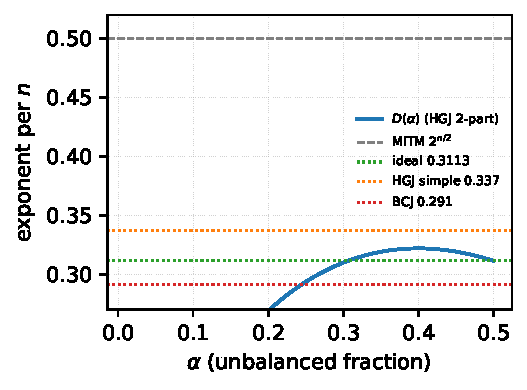
\includegraphics[width=0.9\columnwidth]{figures/fig_representation_exponents}
\caption{The two-way list-size exponent $\log_2 D$ of
Proposition~\ref{prop:two} as a function of the solution weight fraction
(horizontal axis), with the meet-in-the-middle exponent $0.5$ and the
published values $0.3113$, $0.337$ and $0.291$ as reference lines.}
\label{fig:d}
\end{figure}

\section{Why Only Random Inputs?}\label{sec:probes}

\subsection{The assumption behind the bounds}
Every bound above rests on one assumption: the sums of the representations of
a solution are spread fairly evenly over the residues modulo $M$. Then a random
residue $R$ catches about one representation, and the filtered lists have the
sizes in Proposition~\ref{prop:two}. For random numbers this is very plausible.
For a chosen input it can fail badly. If every $a_i$ is a multiple of $M$, for
example, every sum has residue $0$. A filter with $R\ne0$ then keeps nothing,
and a filter with $R=0$ keeps everything, so the filter never shrinks the
search. A worst-case algorithm has to cope with inputs like this.

A natural guess is that some recognisable kind of input is responsible for the
gap. We tested two such guesses with small experiments on six input families:
\begin{itemize}
\item \emph{random}: random numbers of about $n$ bits (density $1$);
\item \emph{dissociated}: numbers whose $2^n$ subset sums are all different;
\item \emph{geometric} and \emph{near-geometric}: powers of two, exactly or with
small random changes;
\item \emph{arithmetic}: numbers in an arithmetic progression;
\item \emph{concentrated}: all numbers multiples of the modulus $M$.
\end{itemize}
Each input has a planted solution of weight $n/2$. Experiment~2 also uses a
seventh family, \emph{dense random}, with small random numbers.

\subsection{Experiment 1: do the representations spread out?}
For the planted solution we computed the residues, modulo $M\approx N$, of all
its $N=\binom{n/2}{n/4}$ two-way representations, and measured the
\emph{coverage}: the fraction of the $M$ residues that receive at least one
representation. If $N$ items land in $N$ residues at random, the expected
coverage is $1-1/e\approx0.63$, so values near $0.6$ mean ``spread like
random''.

At $n=32$ ($N=12{,}870$), the random, dissociated, geometric and near-geometric
families all have coverage between $0.59$ and $0.65$. The arithmetic family
drops to $0.009$ and the concentrated family to $0.0001$. At smaller $n$ the
geometric families were lower ($0.33$--$0.38$ at $n=20$) but rose with $n$. So
the families that look hardest keep the random-like spread. Only the families
with built-in arithmetic structure lose it.

\subsection{Experiment 2: are there too many false matches?}
A filter can also fail by keeping too many \emph{wrong} candidates. For each
input we counted the subsets that reach the target: $T$ with exactly $n/2$
items (true solutions of the expected weight) and $P$ with fewer items (other
subsets that also hit the target and compete in the search). For
$n=12,14,\dots,20$, the dissociated, geometric and near-geometric families
always had $T=1$ and $P=0$, and the random family had $P=0$ except once
($P=1$ at $n=14$). Large values of $P$ appeared only in the arithmetic and
dense random families, which have many solutions anyway.

\subsection{What the experiments say}
Neither guess explains the gap. The inputs that look hardest behave like random
ones in both tests, and the inputs that break the filter are highly structured.
A worst-case input that defeats the technique would have to be unstructured
enough to resist other methods and still concentrate its residues, and we did
not find such a family. These are small experiments, so they rule out
explanations, not algorithms.

\section{The Worst-Case Method and the Open Cases}\label{sec:frontier}
Randolph and W\k{e}grzycki~\cite{rw} turned the representation idea into
worst-case algorithms for many coefficient sets $C$. One of their main tools is
\emph{coefficient shifting}. They write the coefficient set as a \emph{sumset}
\[
C=C_1+C_2=\{c_1+c_2: c_1\in C_1,\ c_2\in C_2\},
\]
and represent each coefficient vector as a sum of a vector over $C_1$ and a
vector over $C_2$. This produces many representations only if some coefficient
can be written as $c_1+c_2$ in at least two ways. For example,
\[
\{0,1\}+\{-3,-2,1,2\}=[\pm3],
\]
where $-2=0+(-2)=1+(-3)$ and $2=0+2=1+1$ each have two representations.
Equal subset sum works too: $\{0,1\}+\{-1,0\}=\{-1,0,1\}$, and $0$ has two
representations.

Their results leave three coefficient sets open: $\{0,1\}$ (subset sum),
$\{-1,1\}$ (Partition) and $[\pm2]=\{-2,-1,1,2\}$. We say that $C=C_1+C_2$ is a
\emph{useful} factorisation if some element of $C$ has at least two
representations $c_1+c_2$.

\begin{proposition}\label{prop:frontier}
None of $\{0,1\}$, $\{-1,1\}$ and $\{-2,-1,1,2\}$ has a useful factorisation.
\end{proposition}

The proof, in Appendix~\ref{app:frontier}, uses only the elementary fact that
$|C_1+C_2|\ge|C_1|+|C_2|-1$. A computer search over all small $C_1,C_2$ inside
$[-3,3]$ agrees (Table~\ref{tab:shift}). So for plain subset sum, coefficient
shifting has nothing to work with. Note that $\{0,1\}$ contains $0$, so having a
zero coefficient is not what matters; what matters is the size and shape of the
set.

\begin{table}[t]
\centering
\caption{Computer search over factorisations $C=C_1+C_2$ with small
$C_1,C_2\subseteq[-3,3]$. ``Useful'' counts factorisations in which some
coefficient has two or more representations.}
\label{tab:shift}
\begin{tabular}{lrr}
\toprule
$C$ & useful & max.\ representations \\
\midrule
$\{0,1\}$ (subset sum) & 0 & 1 \\
$\{-1,1\}$ (Partition) & 0 & 1 \\
$[\pm2]$ & 0 & 1 \\
$\{-1,0,1\}$ (equal subset sum) & 6 & 2 \\
$[\pm3]$ & 4 & 2 \\
$[-2:2]$ & 39 & 3 \\
\bottomrule
\end{tabular}
\end{table}

\section{Conclusion}
The representation technique gets its speed from a simple fact: a solution can
be split in very many ways, so a random filter can throw most of them away and
still keep one. On random inputs this gives about $2^{0.291n}$ steps. The bound
depends on the representations being spread out modulo the filter, which is not
guaranteed for every input. In our experiments, the inputs that look hardest
are spread out like random ones, so the gap is not explained by an obvious
class of bad inputs. The known worst-case method needs a useful factorisation
of the coefficient set, and Proposition~\ref{prop:frontier} shows that subset
sum has none. A worst-case $2^{n/3}$ algorithm for subset sum, or anything below
$2^{n/2}$, would therefore need a different source of extra representations.

\appendices
\section{Derivation of Proposition~\ref{prop:two}}\label{app:two}
Let $x$ be a solution of weight $\ell=\lambda n$, and let $M=\binom{\ell}{\ell/2}$.

\emph{Survivors.} The representations of $x$ are the pairs $(y,x-y)$ where $y$
picks $\ell/2$ of the $\ell$ chosen positions, so there are $M$ of them. Under
the assumption, each $a\cdot y$ has residue $R$ with probability $1/M$, so the
expected number with $a\cdot y\equiv R$ is $M\cdot(1/M)=1$. For each such $y$,
the partner $z=x-y$ has $a\cdot z=b-a\cdot y\equiv b-R$, so it lies in $Z$, and
the pair is found by the search.

\emph{List size.} There are $\binom{n}{\ell/2}$ vectors of weight $\ell/2$. Under
the assumption, about a $1/M$ fraction of them has residue $R$, so
$|Y|\approx\binom{n}{\ell/2}/\binom{\ell}{\ell/2}$, and the same holds for $Z$.

\emph{Exponent.} By the entropy estimate of Section~\ref{sec:prelim},
$\log_2\binom{n}{\lambda n/2}\approx nH(\lambda/2)$ and
$\log_2\binom{\lambda n}{\lambda n/2}\approx \lambda n\,H(1/2)=\lambda n$. So
$\log_2|Y|\approx n\,(H(\lambda/2)-\lambda)$, which is the claim. For
$\lambda=1/2$, $H(1/4)=0.8113$, so the exponent is $0.3113$.

\emph{Equivalent form.} Expanding the entropy,
\[
H(\lambda/2)=1-\tfrac{\lambda}{2}\log_2\lambda-\tfrac{2-\lambda}{2}\log_2(2-\lambda),
\]
so
\[
D(\lambda)=\frac{2}{\lambda^{\lambda/2}(2-\lambda)^{(2-\lambda)/2}}\cdot2^{-\lambda},
\]
which is the form in~\cite[Sec.~4.1]{hgj}. \hfill$\square$

\section{The BCJ Cost Model}\label{app:bcj}
This appendix states the model of~\cite{bcj} that we evaluated. The algorithm
splits the solution three times, into $2$, $4$ and then $8$ pieces. At each
level the pieces may contain extra $+1$ and $-1$ entries that cancel when the
pieces are added. As fractions of $n$, the numbers of $+1$ and $-1$ entries in
one piece at the three levels $\nu,\kappa,\omega$ are
\begin{align*}
N_\nu(1)&=\tfrac14+\alpha, & N_\nu(-1)&=\alpha,\\
N_\kappa(1)&=\tfrac18+\tfrac\alpha2+\beta, & N_\kappa(-1)&=\tfrac\alpha2+\beta,\\
N_\omega(1)&=\tfrac1{16}+\tfrac\alpha4+\tfrac\beta2+\gamma, &
N_\omega(-1)&=\tfrac\alpha4+\tfrac\beta2+\gamma.
\end{align*}
At each level the modulus $M_\chi$ is chosen so that about one representation of
each piece survives, as in Appendix~\ref{app:two}. The list at level $\chi$ then
has size $L_\chi$ equal to the number of vectors with the counts $N_\chi$
divided by the product of the moduli used so far. Let $h_\omega$ be the entropy
of the coefficient distribution at the bottom level, so the bottom lists are
built from half-lists of size $2^{h_\omega n/2}$. The running time is
\[
T=\max\Bigl(2^{h_\omega n/2},\,L_\omega,\,\tfrac{L_\omega^2}{M_\kappa},\,
L_\kappa,\,\tfrac{L_\kappa^2}{M_\nu},\,L_\nu,\,
L_\nu^2\tfrac{M_\nu M_\kappa M_\omega}{2^n}\Bigr).
\]
Each fraction $L^2/M$ is the number of pairs produced when two lists of size
$L$ are merged under a modulus $M$. At the optimum
$(\alpha,\beta,\gamma)\approx(0.027,0.017,0.003)$ the base-list term is
$2^{0.266n}$, below the binding terms, and $T\approx2^{0.291n}$.

\section{Proof of Proposition~\ref{prop:frontier}}\label{app:frontier}

\begin{lemma}\label{lem:sumset}
For finite nonempty sets of integers $A$ and $B$,
$|A+B|\ge|A|+|B|-1$.
\end{lemma}
\begin{proof}
Write $A=\{x_1<\dots<x_p\}$ and $B=\{y_1<\dots<y_q\}$. The $p+q-1$ sums
\[
x_1+y_1<x_1+y_2<\dots<x_1+y_q<x_2+y_q<\dots<x_p+y_q
\]
are strictly increasing, so they are distinct elements of $A+B$.
\end{proof}

Let $C=C_1+C_2$ with both sets nonempty, and suppose some element has two
representations. Then the $|C_1|\,|C_2|$ pairs $(c_1,c_2)$ produce fewer than
$|C_1|\,|C_2|$ distinct sums, so $|C|<|C_1|\,|C_2|$. In particular both
$|C_1|\ge2$ and $|C_2|\ge2$, because if one set has a single element, every sum
has exactly one representation.

\emph{Two-element sets.} Let $C$ be $\{0,1\}$ or $\{-1,1\}$. By
Lemma~\ref{lem:sumset}, $2=|C|\ge|C_1|+|C_2|-1\ge3$, a contradiction.

\emph{The set $[\pm2]$.} Here $|C|=4$, so $|C_1|+|C_2|\le5$ by
Lemma~\ref{lem:sumset}, and $|C_1|\,|C_2|>4$ from above. With both sizes at
least $2$, the only option is sizes $2$ and $3$; say $C_1=\{x_1<x_2\}$ and
$C_2=\{y_1<y_2<y_3\}$. Then $|C_1+C_2|=4=|C_1|+|C_2|-1$. The two increasing
chains
\[
x_1{+}y_1<x_1{+}y_2<x_1{+}y_3<x_2{+}y_3,\qquad
x_1{+}y_1<x_2{+}y_1<x_2{+}y_2<x_2{+}y_3
\]
each list four distinct elements of a set of size four, so both are the whole
set in increasing order. Comparing them term by term gives
$x_1+y_2=x_2+y_1$ and $x_1+y_3=x_2+y_2$. With $d=x_2-x_1$ this means
$y_2-y_1=y_3-y_2=d$, so
\[
C_1+C_2=\{x_1+y_1+kd: k=0,1,2,3\},
\]
an arithmetic progression. But $\{-2,-1,1,2\}$ is not an arithmetic progression,
since its gaps are $1,2,1$. This is a contradiction. \hfill$\square$

\begin{thebibliography}{9}
\bibitem{hs} E. Horowitz and S. Sahni, ``Computing partitions with applications
to the knapsack problem,'' \emph{J. ACM}, vol.~21, no.~2, pp.~277--292, 1974.
\bibitem{ss} R. Schroeppel and A. Shamir, ``A $T=O(2^{n/2})$, $S=O(2^{n/4})$
algorithm for certain NP-complete problems,'' \emph{SIAM J. Comput.}, vol.~10,
no.~3, pp.~456--464, 1981.
\bibitem{hgj} N. Howgrave-Graham and A. Joux, ``New generic algorithms for hard
knapsacks,'' in \emph{EUROCRYPT}, 2010; IACR ePrint 2010/189.
\bibitem{bcj} A. Becker, J.-S. Coron, and A. Joux, ``Improved generic algorithms
for hard knapsacks,'' in \emph{EUROCRYPT}, 2011; IACR ePrint 2011/474.
\bibitem{chen} X. Chen, Y. Jin, T. Randolph, and R. A. Servedio, ``Subset sum
in time $2^{n/2}/\mathrm{poly}(n)$,'' in \emph{RANDOM}, 2023; arXiv:2301.07134.
\bibitem{rw} T. Randolph and K. W\k{e}grzycki, ``Beating meet-in-the-middle for
subset balancing problems,'' arXiv:2511.10823, 2025.
\bibitem{bbss} X. Bonnetain, R. Bricout, A. Schrottenloher, and Y. Shen,
``Improved classical and quantum algorithms for subset-sum,'' in
\emph{ASIACRYPT}, 2020; IACR ePrint 2020/168.
\end{thebibliography}
\end{document}
